\begin{figure}[htpb]
\centering\capstart{}
\subfloat[\(\Re\big\{\pixel{W^{\Phi}}\big\}\)] % chktex 21
{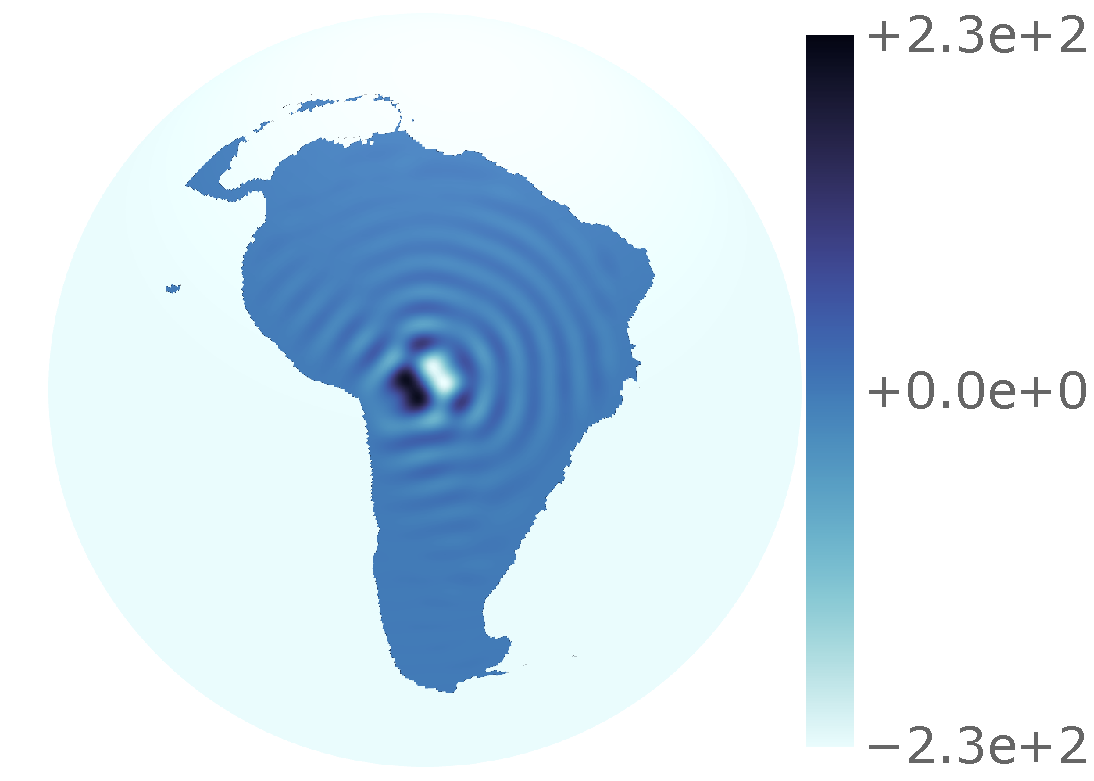
\includegraphics[trim={4 7 3 6},clip,width=.5\textwidth]{slepian_wavelet_coefficients_south_america_3B_2jmin_scaling_2smoothed_L128_res512_real.pdf}}
\hfill
\subfloat[\(\Re\big\{\pixel{W^{\Psi^{2j}}}\big\}\)] % chktex 21
{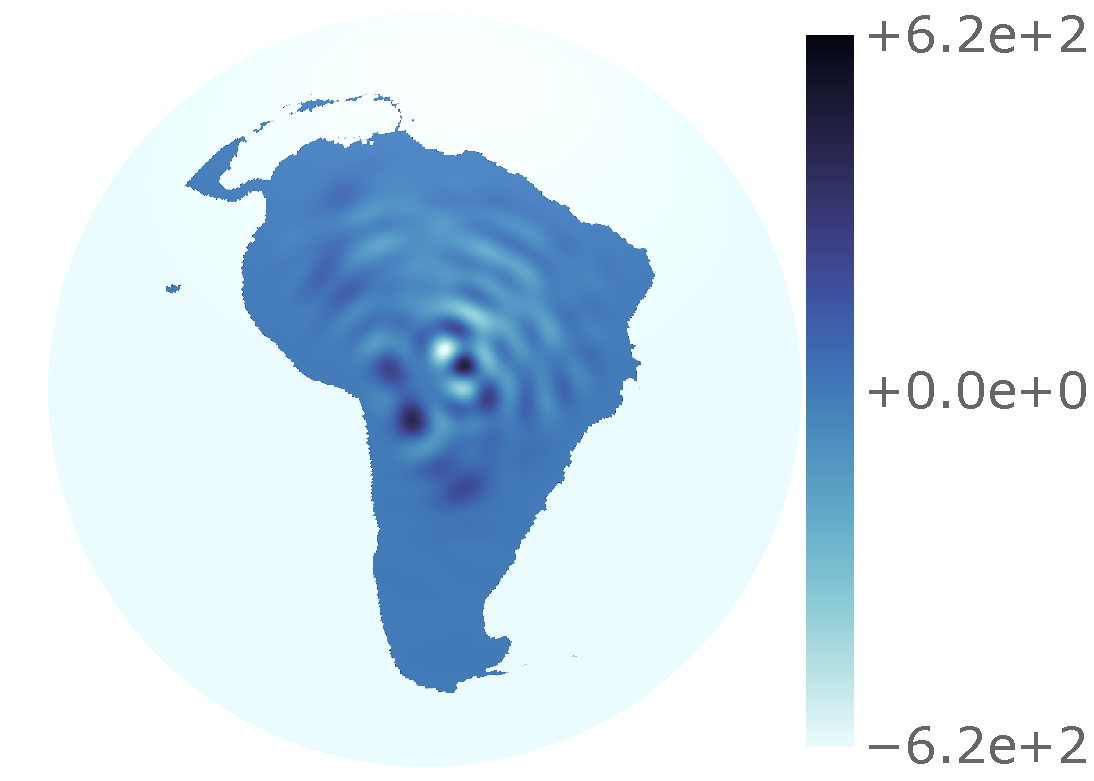
\includegraphics[trim={4 7 3 6},clip,width=.5\textwidth]{slepian_wavelet_coefficients_south_america_3B_2jmin_2j_2smoothed_L128_res512_real.pdf}}
\newline
\subfloat[\(\Re\big\{\pixel{W^{\Psi^{3j}}}\big\}\)] % chktex 21
{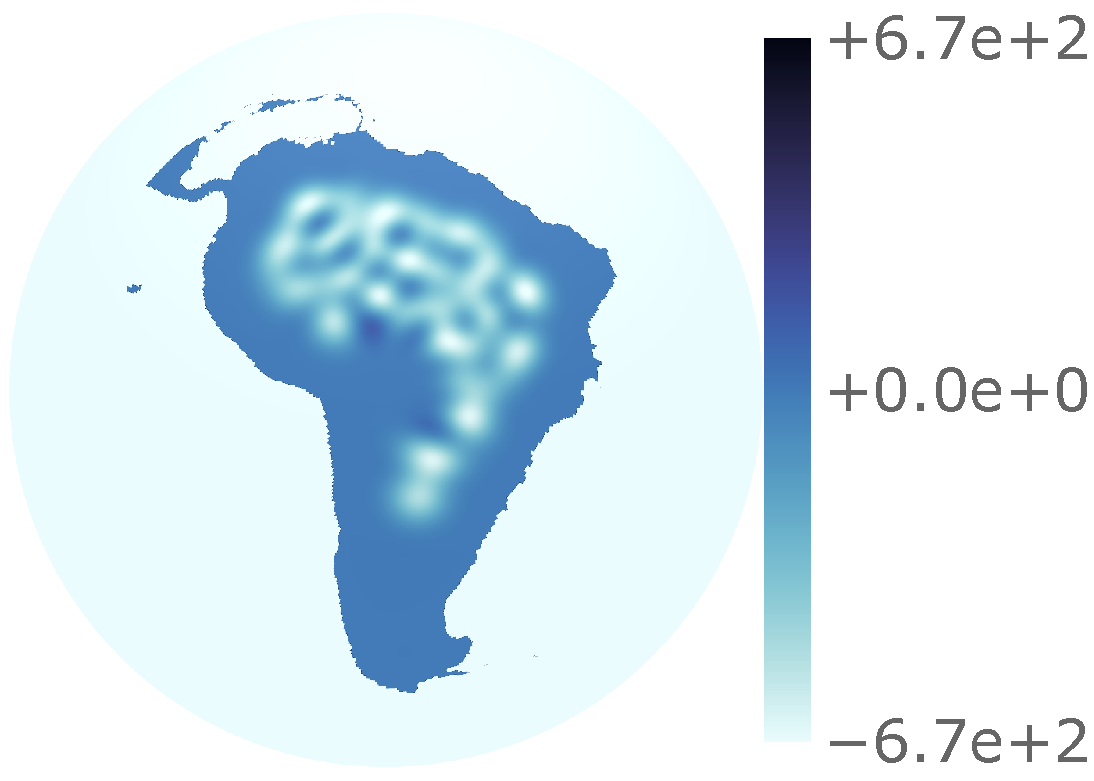
\includegraphics[trim={4 7 3 6},clip,width=.5\textwidth]{slepian_wavelet_coefficients_south_america_3B_2jmin_3j_2smoothed_L128_res512_real.pdf}}
\hfill
\subfloat[\(\Re\big\{\pixel{W^{\Psi^{4j}}}\big\}\)] % chktex 21
{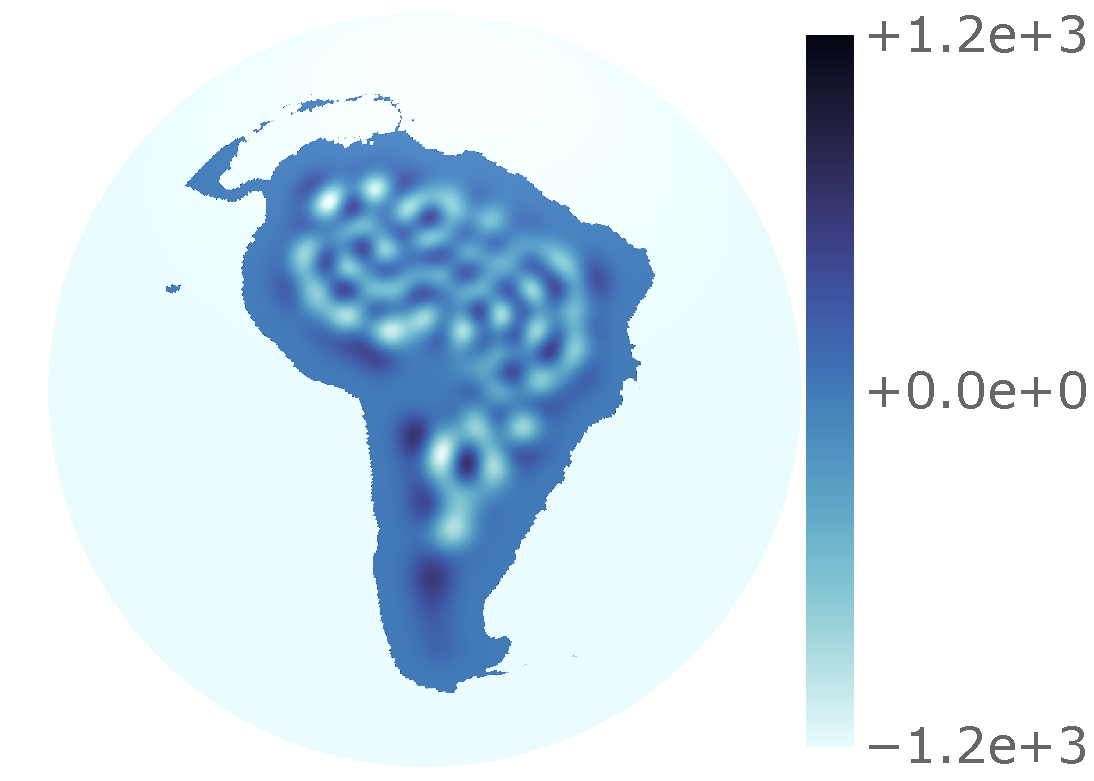
\includegraphics[trim={4 7 3 6},clip,width=.5\textwidth]{slepian_wavelet_coefficients_south_america_3B_2jmin_4j_2smoothed_L128_res512_real.pdf}}
\newline
\subfloat[\(\Re\big\{\pixel{W^{\Psi^{5j}}}\big\}\)] % chktex 21
{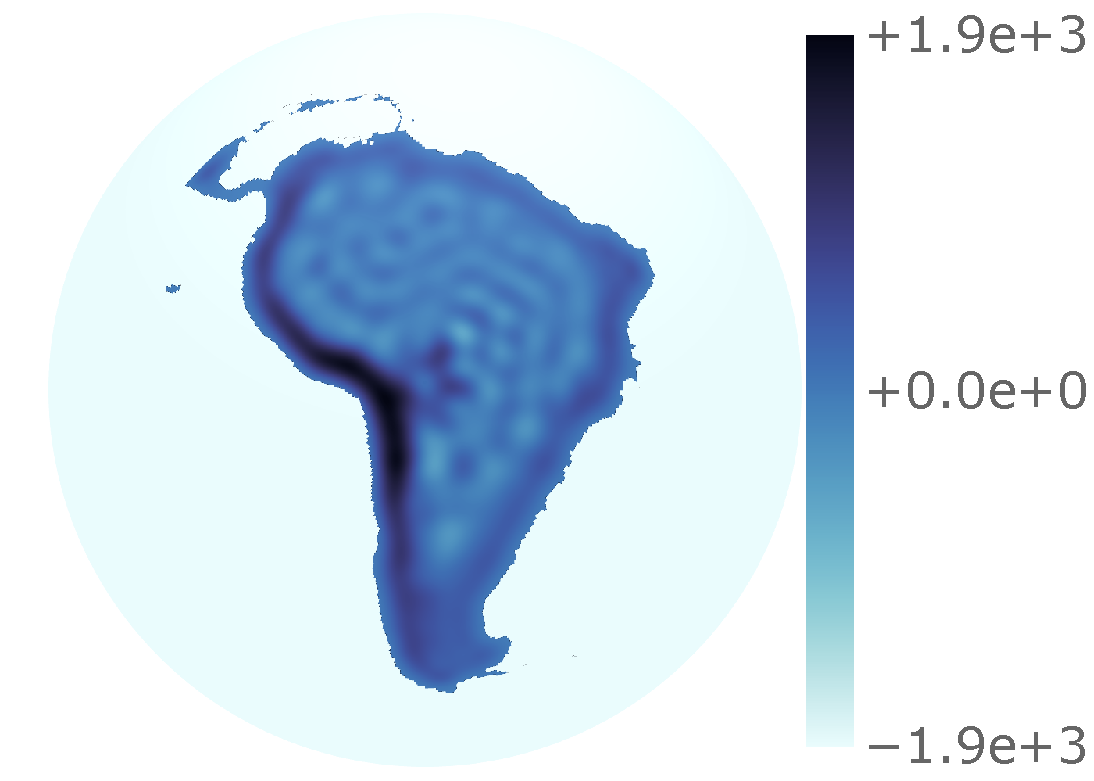
\includegraphics[trim={4 7 3 6},clip,width=.5\textwidth]{slepian_wavelet_coefficients_south_america_3B_2jmin_5j_2smoothed_L128_res512_real.pdf}}
\hfill
\subfloat[\(\Re\big\{\pixel{W^{\Psi^{6j}}}\big\}\)] % chktex 21
{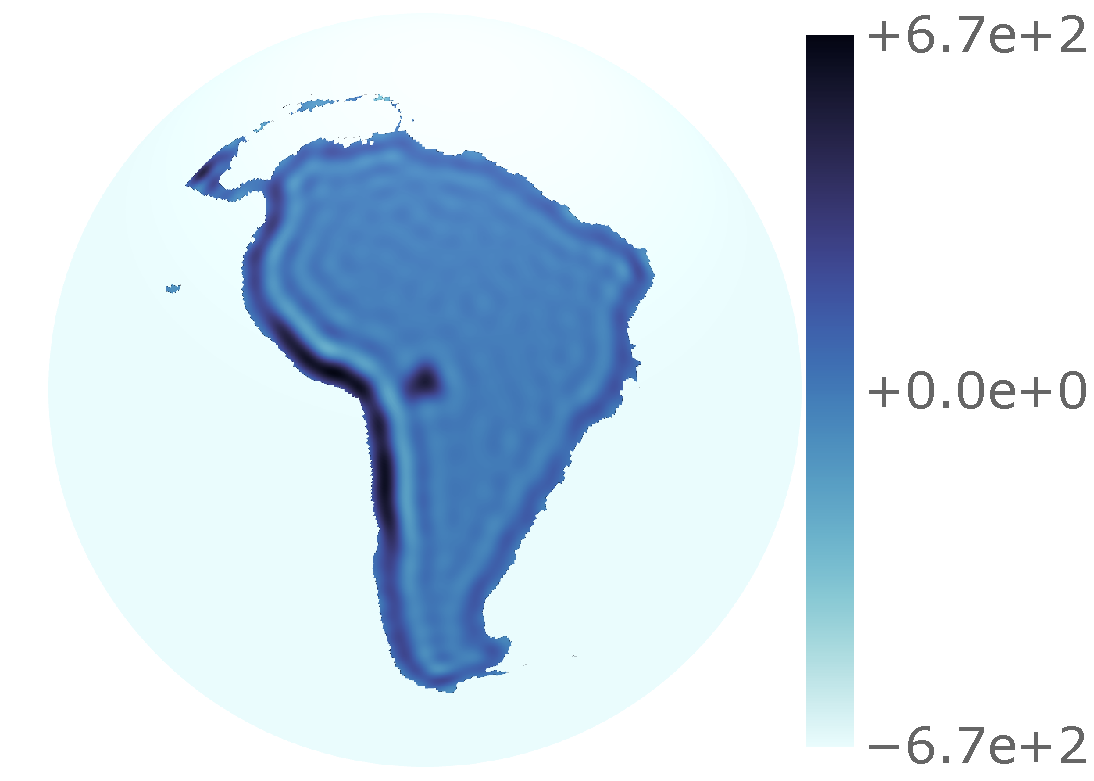
\includegraphics[trim={4 7 3 6},clip,width=.5\textwidth]{slepian_wavelet_coefficients_south_america_3B_2jmin_6j_2smoothed_L128_res512_real.pdf}}
\caption[
The Slepian wavelet coefficients of a map of South America
]{
The scale-discretised wavelet transform of the topographic map of South America for parameters \(\lambda=3\), \(J_{0}=2\), and bandlimit \(L=128\); \ie{} with the wavelets shown in \cref{fig:chapter4_slepian_wavelets}.
Spatially localised, scale-dependent features of the bandlimited signal may be extracted by the wavelet coefficients given by the wavelet transform.
The scaling coefficients are given in the top left plot, while the wavelet coefficients at scales \(j \in \set{2, 3, 4, 5, 6}\) are shown left-to-right, top-to-bottom.
}\label{fig:chapter4_slepian_wavelet_coefficients}
\end{figure}
